\chapter{Codesigning Humanoid Robots with Deep Reinforcement Learning}
\label{chp:contrib_CodesignRL}

This chapter will describe the process of designing the codesign loop, exploiting the theoretical foundation regarding deep reinforcement learning and evolutionary algorithms presented in \cref{chp:back_RLGA} and the conditioning of \ac{RBDA}s presented in \cref{chp:contrib_ABA} via a hardware accelerated physics simulator.

\section{Reinforcement Learning Problem Definition}

In the reinforcement learning loop of the codesign process, the aim is to find a policy $\pi$ that maximizes the expected return $J(\pi)$, which is defined as the expected sum of rewards over an infinite horizon:

\begin{equation}
    J(\pi) = \mathbb{E} \left[ \sum_{t=0}^{\infty} \gamma ^t r_t \right]
\end{equation}

\dots

All the \ac{RL} trainings in this work have been performed on the \texttt{IITBMP014SRV001} machine whose specifications are reported in \cref{tab:rl_machine}.

\begin{table}[h]
    \centering
    \label{tab:rl_machine}
    \caption{\texttt{IITBMP014SRV001} Server Specifications}
    \begin{tabular}[h]{l c}
        \toprule
        \textsc{Component} & \textsc{Specification}                                            \\
        \midrule
        \textbf{CPU}       & \begin{small}AMD EPYC 7513 32-Core Processor @ 2.60GHz\end{small} \\
        \textbf{GPU}       & \begin{small}NVIDIA A100 80GB PCIe                   \end{small}  \\
        \textbf{RAM}       & \begin{small}1024GB DDR4-3200                        \end{small}  \\
        \textbf{OS}        & \begin{small}Ubuntu 20.04.3 LTS                      \end{small}  \\
        \textbf{Kernel}    & \begin{small}5.15.0-86-generic                       \end{small}  \\
        \bottomrule
    \end{tabular}
\end{table}

\subsection{Cartpole swingup task}
For the cartpole swing-up task, the aim is to find a policy $\pi$ that is able to balance the pole on the cart, which is moving on a rail, and then swing-up the pole to the upright position. The reward function is defined as a function of the state of the system, which is composed of the position of the cart $x$, the velocity of the cart $\dot{x}$, the angle of the pole $\theta$ and the angular velocity of the pole $\dot{\theta}$:

\begin{equation}
    r = \begin{cases}
        1 & \text{if } \left| \theta \right| < \theta_{\text{max}} \\
        0 & \text{otherwise}
    \end{cases}
\end{equation}

where $\theta_{\text{max}}$ is the maximum angle of the pole from the vertical position.

\begin{table}
    \centering
    \label{tab:cartpoleswinguptaskspacedef}
    \begin{tabular}{l c}
        \toprule
        \textsc{Space}                  & \textsc{Projection Space} \\
        \midrule
        Action Space $\mathcal{A}$      & $\mathbb{R}$              \\
        Observation Space $\mathcal{S}$ & $\mathbb{R} ^{4}$         \\
        Reward Space $\mathcal{R}$      & $[0,1]$                   \\
        \bottomrule
    \end{tabular}
    \caption{Cartpole Swingup Task -- Space Definition}
\end{table}


\subsection{Humanoid locomotion task}
The humanoid walking task is without a doubt one of the most challenging tasks in the field of robotics. The task aims to find a policy $\pi$ that is able to make the robot walk forward in a possibly \textit{human-like} motion. Given its high complexity, constituted by the necessity of controlling a large number of joints, which drastically increases the dimensionality of the problem and the need to design a contact model that can simulate the interaction between the robot and the environment, yet allowing the algorithm to be able to predict the agent's behavior as described in \cref{sec:back_contacts},

The action space is defined as:

\begin{equation}
    \mathcal{A} = \left\{ a \in \mathbb{R} ^{23} \mid -1 \leq a_i \leq 1 \right\}
\end{equation}

where $a_i$ is the $i$-th joint desired position, which is then converted to a torque via a PD controller and then clipped to the maximum torque of the joint.

The observation space is defined as:

\begin{equation}
    \mathcal{S} = \left\{ s \in \mathbb{R} ^{80} \mid -\infty \leq s_i \leq \infty \right\}
\end{equation}

and it is composed of the elements listed in \cref{tab:walkingobs}.

\begin{table}
    \centering
    \label{tab:walkingobs}
    \begin{tabular}{l c}
        \toprule
        \textsc{Observation} & \textsc{Dimension} \\
        \midrule
        Base Position        & $\mathbb{R} ^{3}$  \\
        Joints Positions     & $\mathbb{R} ^{23}$ \\
        Joints Velocities    & $\mathbb{R} ^{23}$ \\
        Actuation Torques    & $\mathbb{R} ^{23}$ \\
        Contact Points       & $\mathbb{R} ^{1}$  \\
        Target Position      & $\mathbb{R} ^{3}$  \\
        \bottomrule
    \end{tabular}
    \caption{Humanoid Walking Task -- Observation Space}
\end{table}

Rewards, actions, and observations are then normalized to the range $[0,1]$ in order to make the learning process more stable and to avoid the need to tune the reward function for different robots. The \cref{tab:walkingtaskspacedef} summarizes the definition of the spaces used in the \ac{RL} framework.

\begin{table}
    \centering
    \begin{tabular}{l c}
        \toprule
        \textsc{Space}                  & \textsc{Projection Space} \\
        \midrule
        Action Space $\mathcal{A}$      & $\mathbb{R} ^{23}$        \\
        Observation Space $\mathcal{S}$ & $\mathbb{R} ^{75}$        \\
        Reward Space $\mathcal{R}$      & $[0,1]$                   \\
        \bottomrule
    \end{tabular}
    \caption{Humanoid Walking Task -- Space Definition}
    \label{tab:walkingtaskspacedef}
\end{table}


Hyperparameter tuning is a crucial part of the \ac{RL} framework, and it is often the most time-consuming part of the process. In this work, the hyperparameters were tuned using \textit{Optuna} \cite{akiba_optuna_2019}, a hyperparameter optimization framework, which uses Tree-structured Parzen Estimator (\ac{TPE}) sampler with a median pruner, that models the objective function and suggests the next set of hyperparameters to evaluate. The hyperparameters that were tuned are the following:

\begin{itemize}
    \item Time Horizon
    \item Minibatch Size
    \item Number of Minibatches
    \item Number of Epochs
    \item Clipping
    \item Discount Factor $\gamma$
    \item GAE Parameter $\lambda$
    \item Value Function Coefficient
    \item Entropy Coefficient $\beta$
    \item Learning Rate
    \item Network Architecture
\end{itemize}

which resulted in in values reported in \cref{tab:ppohyperparameters}.


\begin{table}[h]
    \centering
    \label{tab:ppohyperparameters}
    \begin{tabular}{ll}
        \toprule
        \textsc{Parameter}          & \textsc{Value}          \\
        \midrule
        \multicolumn{2}{c}{\textbf{Training Parameters}}      \\
        Time Horizon                & $2048$                  \\
        Minibatch size              & $4096$                  \\
        Num Minibatch               & $32$                    \\
        Number of Epochs            & $10$                    \\
        \midrule
        \multicolumn{2}{c}{\textbf{PPO Algorithm Parameters}} \\
        Clipping                    & $0.3$                   \\
        KL Target                   & Not Implemented         \\
        KL Initialization           & Not Implemented         \\
        Discount Factor $\gamma$    & $0.99$                  \\
        GAE Parameter $\lambda$     & $0.95$                  \\
        \midrule
        \multicolumn{2}{c}{\textbf{Coefficients}}             \\
        Value Function Coefficient  & $1.0$                   \\
        Entropy Coefficient $\beta$ & $0.01$                  \\
        \midrule
        \multicolumn{2}{c}{\textbf{Optimization Parameters}}  \\
        Learning Rate               & $0.0003$                \\
        Maximum Gradient Norm       & $0.5$                   \\
        \bottomrule
    \end{tabular}
    \caption{Proximal Policy Optimization Hyperparameters}
\end{table}

Given the high complexity of the problem, the network architecture composed of two separate networks, one for the policy and one for the value function, has been enlarged in order to increase the capacity of the network to learn the task and to avoid the need of a large number of training iterations.

The policy network is composed of two hidden layers of size $64$ and $64$ respectively, with a \ac{ReLU} activation function. The value function network is composed of two hidden layers of size $64$ and $64$ respectively, with a \ac{ReLU} activation function. The output of the policy network is a vector of size $23$. The output of the value function network is a scalar, which is then used to compute the advantage function. The \cref{fig:rlarchitecture} shows the architecture of the \ac{RL} framework, for a better visualization of the network architecture, the number of neurons has been divided by $128$.

\begin{figure}[h]
    \centering
    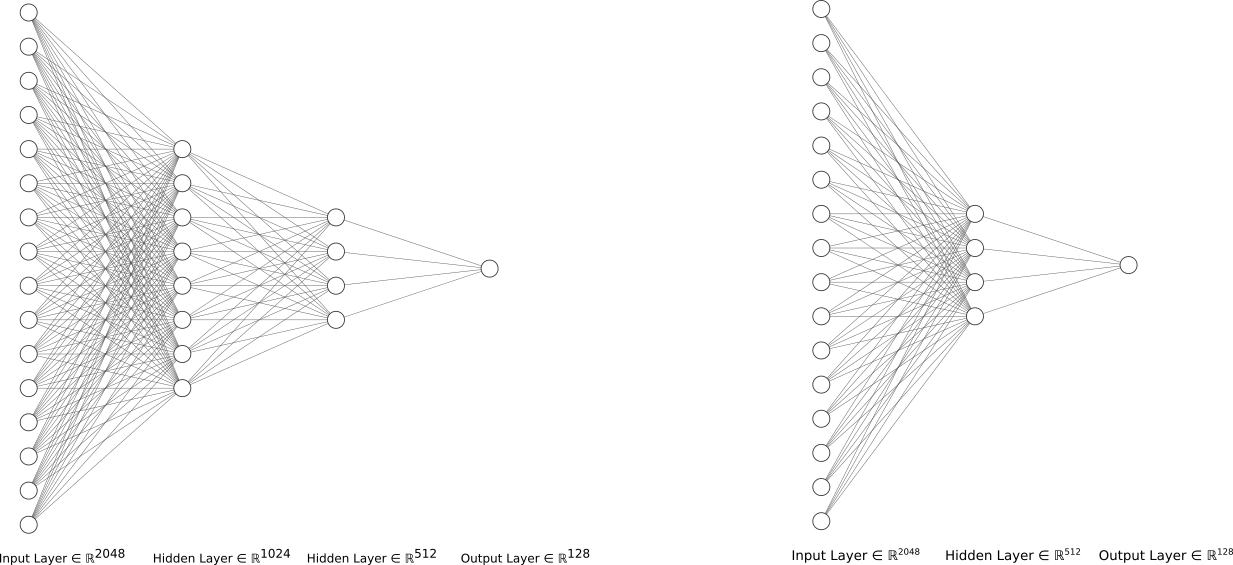
\includegraphics[width=0.8\textwidth]{Images/rl_architecture.png}
    \caption{TOBE CHANGED RL Framework Architecture: Actor-Critic Network}
    \label{fig:rlarchitecture}
\end{figure}

The \ac{RL} framework has been implemented using the \textit{Stable Baselines 3} library \cite{raffin_stable-baselines3_2021}. The \ac{RL} framework has been trained for $10$M steps, which given the episodic length, corresponds to $10$ epochs. The INSERT FIGURE below represents the main metrics collected in the training process. In particular, the figure shows the mean reward, the mean episode length, the mean episodic reward, the approximated KL divergence, and the explained variance.


\section{Evolutionary Algorithm Core}
\label{sec:EvolutionAlgo}


The evolutionary algorithm has been used in the codesign loop to select motor parameters from a set of possible values. The evolutionary algorithm has been implemented using the \textit{DEAP} library CITE.

The motor set of parameters is composed of three main components: motor inertia, motor viscous friction, and gear ratio. This choice has been made in order to keep the number of parameters low, in order to reduce the computational cost of the optimization process. The decision process is then repeated for each motor of the robot, which means that the total number of combination are:

\begin{equation}
    H = \binom{n + k - 1}{k} = \binom{23 + 3 - 1}{3} = \frac{25!}{3! 22!} = 2300
\end{equation}

where $n$ is the number of motors and $k$ is the number of parameters for each motor. In order to reduce the computational expense, we decided to focus on four crucial motors of the robot, which are the motors of the legs. This choice has been made because the legs are the main component of the robot that interacts with the environment, and therefore the choice of the motor parameters has a great impact on the performance of the robot. The total number of combinations is then reduced to:

\begin{equation}
    H = \binom{n + k - 1}{k} = \binom{4 + 3 - 1}{3} = \frac{6!}{3! 3!} = 20
\end{equation}

The evolutionary algorithm has been used to select the motor parameters from the set of possible values. The set of possible values for each parameter is shown in the \cref{tab:motorparams}.

\begin{table}[h]
    \centering
    \begin{tabular}{c c c c}
        \toprule
        \textsc{Motor} & \textsc{Inertia} $[k\mathrm{gm}^2]$ & \textsc{Gear Ratio} & \textsc{Viscous Friction} $[\mathrm{N}s\mathrm{rad}^{-1}]$ \\
        \midrule
        \textbf{S}     & $0.0001$                            & $1/100.0$           & $0.1$                                                      \\
        \textbf{M}     & $0.001$                             & $1/100.0$           & $0.15$                                                     \\
        \textbf{L}     & $0.001$                             & $1/160.0$           & $0.2$                                                      \\
        \bottomrule
    \end{tabular}
    \caption{Motor Set Parameters}
    \label{tab:motorparams}
\end{table}


After a preliminary analysis of the problem, the following parameters have been selected:

\begin{table}
    \centering
    \begin{tabular}{ll}
        \toprule
        \textsc{Parameter}    & \textsc{Value} \\
        \midrule
        Population Size       & $100$          \\
        Number of Generations & $100$          \\
        Crossover Probability & $0.5$          \\
        Mutation Probability  & $0.2$          \\
        \bottomrule
    \end{tabular}
    \caption{Evolutionary Algorithm Hyperparameters}
\end{table}

Given the single objective of the optimization problem, the \ac{NSGA}-III algorithm has been selected as the evolutionary algorithm, as it allows us to find a set of solutions that are all Pareto optimal.


\section{Humanoid Robots Codesign Loop}
\label{sec:Codesign}

The problem of humanoid robot codesign can be formalized as a reinforcement learning problem, where the agent is the robot, together with a nonlinear optimization of some hardware parameters, in the case discussed in this work this role is played by an evolutionary algorithm.

The first step of the codesign loop involves some initial design choices, which are then used to create the initial population of the evolutionary algorithm. Then the population gets evaluated running in parallel the \ac{RL} framework for each individual of the population. The evaluation process is repeated for several generations, after which the best individual is selected and its parameters are used to update the robot design. The process is then repeated until the robot reaches the desired target fitness or when it reaches the maximum number of generations.

For the evaluation, the reward coming from the \ac{RL} training process is used as the fitness function of the evolutionary algorithm. The fitness function is then normalized to the range $[0,1]$ in order to make the optimization more stable.
